\documentclass[12pt,a4paper]{article}
\usepackage[utf8]{inputenc}
\usepackage[swedish]{babel}
\usepackage{amsmath}
\usepackage{amsfonts}
\usepackage{amssymb}
\usepackage{graphicx}
\usepackage{float}
\usepackage[hidelinks]{hyperref}
\usepackage[backend=biber,style=numeric,sorting=none]{biblatex}
\addbibresource{cites.bib}
\usepackage{caption}
\captionsetup[figure]{name=Figur}

\author{Alfred Yrelin\\Josef Svensson\\Philip Åkerfeldt}
\title{Är du en historiemästare?}
\begin{document}
\maketitle
\newpage
\tableofcontents
\pagebreak

\section{Inledning}
Vem vill inte kunna avgöra diskussioner med sina vänner med argumentet "Jag är i alla fall bäst på ..."? 
Att tävla är något som de allra flesta säkerligen tycker är både roligt och socialt; om målet är att vinna eller bara ha kul varierar men tävlingskänslan finns kvar oavsett agenda. Att kunna ha denna tävlingskänsla och en källa för nöje så förmånligt i sin telefon är något som vi tror att spel som Quizkampen\cite{quiz} och Wordfeud har blivit så populära. Vi eftersträvar att skapa ett spel som kan framkalla samma tävlingskänsla och nöje som tidigare nämnda spel. Ett spel som går ut på att ordna historiska händelser relativt till andra händelser. Spelet utvecklas till Android med en backend som drar nytta av Google App Engines skalbarhet för att ge applikationen möjlighet att växa i takt med användarantalet. Automatisk frågehämtare och balansering är bara några av de sakerna som kommer karaktärisera spelet.


\section{Förutsättningar}

\subsection{Bakgrund}
Applikationsutveckling för mobila enheter är ett spännande område som växer\cite{trendforce} och det operativsystem som sålde mest enheter under första kvartalet av 2015 var Android. 

\subsubsection{Turbaserade multiplayerspel för mobiltelefoner}
Wordfeud och Quizkampen är två populära turbaserade multiplayerspel där Quizkampen har 45 miljoner användare globalt\cite{quiz} och Wordfeud har mellan 10-50 miljoner nedladdningar enbart på Androidplattformen\cite{wordfeud}. Dessa spel gör det möjligt att utmana vänner eller slumpmässiga personer på en match som spelas i omgångar. När en spelare spelar sin omgång får dess motståndare vänta på sin tur, vilket gör att en match kan pågå i flera dagar.
\paragraph{Quizkampen}
är ett frågesports-spel där spelarna svarar på frågor under 6 ronder med tre frågor i varje rond. Spelarna svarar på samma frågor och spelarna väljer en av tre slumpade kategorier varannan rond. Matchen avslutas när sista rundan är spelad och det är även då  en vinnare avgörs. \cite{aboutquiz}


\subsubsection{Turbaserade sällskapsspel}

Frågesportspel i sällskapsspelsform är och har länge varit ett populärt sätt att umgås på\cite{tp}. Det är många som till exempel har spelat \textit{Trivial Pursuit} (TP) (kanske speciellt 84-års utgåva, som återfinns lite här och där). Sällskapsspelet \textit{När då då?} är ett spel som liknar TP på det sättet att den spelare som först svarar rätt på flest frågor förmodligen vinner. Det är ett väldigt enkelt spelkoncept men det utnyttjar också en ganska fundamental egenskap: spelarens vilja att visa sig smartast. Det är förmodligen detta som gör den här typen av spel så populära.

\subsection{Syfte}
Det är projektets syfte är att utveckla och distribuera en spelapplikation för mobila enheter. I det här projektet ska en applikation utvecklas som ger flera användare möjlighet att interagera med varandra.

Spelet som utvecklats går ut på att två användare får tävla om vem som har bäst koll på när olika historiska händelser ägde rum. Varje spelare får ett antal händelser som denne sedan ska sortera i kronologisk ordning. Spelaren som sorterar flest händelser rätt vinner. Förutom rent nöje så ger spelet också användaren möjlighet att få bättre koll på historien, applikationen kan alltså också användas i utbildningssammanhang.

\subsection{Mål}
Det finns tre stora delar i det här projektet som kan ses som projektets primära mål. Målet vi ser framför oss är en mobilapplikation i form av ett spel som kommer köras på en server som kommer sköta all kommunikation mellan klienten och sig själv. Målet vi har innefattar även en automatisk informationshämtning som ska har som syfte att fylla på vår databas med nya frågor. Informationshämtningen kommer inte säkert vara helt automatiskt utan kanske mer semi-automatiskt där ett steg i informationshämtningen kommer kräva ett mänskligt interagerande. Detta för att godkänna frågorna till databasen. 


\subsubsection{Mobilapplikation}
En mobilapplikation till först och främst Android ska utvecklas. Om det finns tid kommer också en version för iOS att utvecklas. Mobilapplikationen är det enda som användaren i slutändan kommer se, därför är gränssnittet extra viktigt i den här delen. 

Applikationen till Android skrivs i Java och gränssnittet skrivs med hjälp av xml-markup.

\subsubsection{Server}
För att flera spelare ska kunna interagera med varandra så behövs det en server. En server gör också att frågorna som finns i spelet kommer kunna uppdateras kontinuerligt.

Servermjukvaran skrivs i programspråket Go \cite{golang} och körs på Googles molntjänst App engine.

\subsubsection{Google App Engine} 
Google App Engine är en \textit{Platform as a service}, vilket är en servicemodell för moltjänster. Det bygger på att användaren bygger en programvara med hjälp av färdigbyggda bibliotek och verktyg som leverantören tillhandahåller. Programet man bygger i App Engine körs på googles infrastruktur och är uppbyggt så att man kan utöka antalet användare närmast obegränsat. Flera stora företag har använt sig av App Engine när de lanserat produkter bland annat Coca Cola, Rovio och Best Buy. \cite{googleappenginecustomers}

\subsubsection{Automatisk informationshämtning}
För att göra spelet så intressant som möjligt behövs det många frågor. Ett sätt att skapa många frågor är att utveckla mjukvara som kan hämta information och sätta ihop frågor automatiskt. 

Målet med den automatiska informationshämtningen är ett delsystem som läser in delar av Wikipedia eller andra källor och kopplar samman årtal och händelser automatiskt. Det här systemet behöver också ett administrativt gränssnitt så att en administratör på ett snabbt vis kan korrekturläsa frågorna innan de används.

\subsection{Motivation}
Det finns många mobilspel som handlar om att två personer möts och mäter sina färdigheter inom ett visst område. Exempel på applikationer är Quizkampen och Wordfeud är toppar säljlistorna för Androidspel \cite{appsalesrating}. Dessa spel följer en ganska enkel struktur och den bygger på att två personer kan möta varandra, svara på frågor eller lägga ord och på så sätt få poäng som sen kommer avgöra en vinnare mellan de tävlande. Enligt säljstatistiken som nämndes tidigare är detta koncept något som är attraktivt för många användare. Spelet, vars utveckling beskrivs i rapporten, kommer kombinerar koncepten från tidigare nämnda spel; med att både svara på frågor samt att lägga in saker på sin rätta plats. 

En liknande version av det här spelet har också visat sig vara populär i form av sällskapsspel (\textit{När-då-då?})\cite{nardada}, därför är hoppet högt om att också den här applikationen ska bli populär. Det finns för tillfället ingen variant av det här spelkonceptet till Android vilket ses som en bra chans att ta enligt utvecklingsteamet.

\subsection{Lägesbeskrivning}
Det finns ett spel för iOS, \textit{Historiekampen}\cite{historiekampen} som också handlar om att lägga in händelser korrekt på en tidslinje. En nackdel som den befintliga iOS-versionen har är att användaren endast ser årtal på sin tidslinje, och inte vilka händelser som ligger där.

Historiekampen är ett spel som mekaniskt sett liknar sällskapsspelet \textit{När då då?} väldigt mycket. En spelares tur går till så att denne får en fråga som ska placeras på spelarens tidslinje. Vid första frågan finns det en årtalsreferens utlagd, vid nästa fråga finns det två referenser (den första plus årtalet för frågan som precis placerades) och så vidare. I Historiekampen kan en spelare välja att antingen lägga en fråga till, eller avsluta sin runda och därmed låsa frågorna. Skulle spelaren svara fel på en fråga förlorar denne alla frågor som har placerats den rundan.

\textbf{vad vi ska göra (varför vi är bättre än dom andra):} 
OKLART VART DENNA SKA LIGGA

Spelet som utvecklats liknar Historiekampen rent konceptuellt. Spelmekaniken är dock annorlunda då varje match och varje runda behandlas annorlunda. I \textbf{VÅRT SPEL} får varje spelare ett paket med fem frågor (som visas en i taget) vilket spelaren ska placera i rätt ordning. oavsett om spelaren lyckas eller inte så går turen efter fem frågor över till motståndaren. När fem rundor har spelats vinner den spelare som har svarat rätt på flest frågor totalt. 

En viktig detalj som skiljer det här spelet från Historiekampen är faktumet att spelaren ser beskrivningen av händelserna som denne placerat, och inte årtalen. \textbf{VÅRT SPEL} handlar alltså mer om att relatera händelser till varandra (dog Palme efter andra världskriget?) än att veta vilket årtal det skedde.

Med den semi-automatiska frågehämtaren som kan anpassas för olika informationskällor är det relativt enkelt att hämta nya frågor. Vår app balanseras också under spelets gång och på så sätt kan alla spelare känna sig bekväma med frågorna som ställs. Balanseringen i spelet kan även byggas ut och göras mer avancerad om användarna skulle ge kritik på hur frågorna kategoriseras. Det finns egentligen inga gränser för hur avancerad balansering kan göras vilket är ett stort plus som skiljer oss från konkurrenterna.

\subsection{Frågeställningar}

\subsubsection{Tekniska problem}
Det finns vissa delar i det här systemet som blir mer avancerade att lösa än andra delar. Här listas några av dessa.
\begin{itemize}
\item Eftersom applikationen ska hämta information att göra frågor av automatiskt så måste ett sådant system konstrueras. En svårighet i detta är att se till så att systemet blir tillräckligt smart för att avgöra vad som kan användas som frågor och inte.
\item Det behövs en ganska stor databas för att hantera både användare och frågor. Det här är någonting som projektmedlemmarna inte har arbetat med i så stor skala förut.
\item Det krävs nätverkskommunikation med säkerhet och användaridentifiering. App Engine har användbara funktioner för delar av detta.
\item Spelet ska anpassa svårighetsgraden automatiskt så någon form av maskininlärning behövs. Tanken är att frågorna ska ha en svårighetsgrad som justeras automatiskt beroende på hur ofta de läggs rätt. Här måste det också tas hänsyn till hur resten av brädet ser ut vid tillfället.
\item Ett system för att rangordna spelare så att en topplista kan visas behövs.
\end{itemize}

\section{Genomförande}

\subsection{Metoder}
Ett antal olika verktyg kommer att användas för att möjliggöra detta projekt. För utvecklingen och simulering av android-applikationen kommer Android Studio användas. Detta är ett kraftfullt verktyg som på ett smidigt sätt kan simulera applikationen i olika valbara miljöer i form av layouts för olika mobiltelefoner. \cite{androidstudio}\\
Google App Engine används lokalt för att simulera serverapplikationen. I skarpt läge kommer App Engine även användas, men då i Googles moln. App engine är ett värdefullt verktyg i vår utveckling med den enkla förklaringen att de tjänster som erbjuds när man utvecklar och körs sina applikationer via denna motor är otroligt värdefulla. Det är bland annat lätt att underhålla applikationen och skala när trafiken och datan kräver det. \cite{googleappengine}\\
Wikipedia används som informationskälla för frågorna som spelet presenterar för användarna. Denna informationskälla används primärt under utvecklingsfasen och kommer mer stor sannolikhet att bytas ut mot andra informationskällor vid ett senare skede alternativt innan produkten färdigställs.\\
Git används för att synkronisera projektets filer mellan utvecklarna. Ett privat repo på Bitbucket\footnote{http://www.bitbucket.org} används till detta.\\
Google Hangouts används för kommunikation när gruppmedlemmarna är på olika fysiska platser.

\subsection{Systemstruktur}

\begin{figure}[H]
	\begin{centering}
	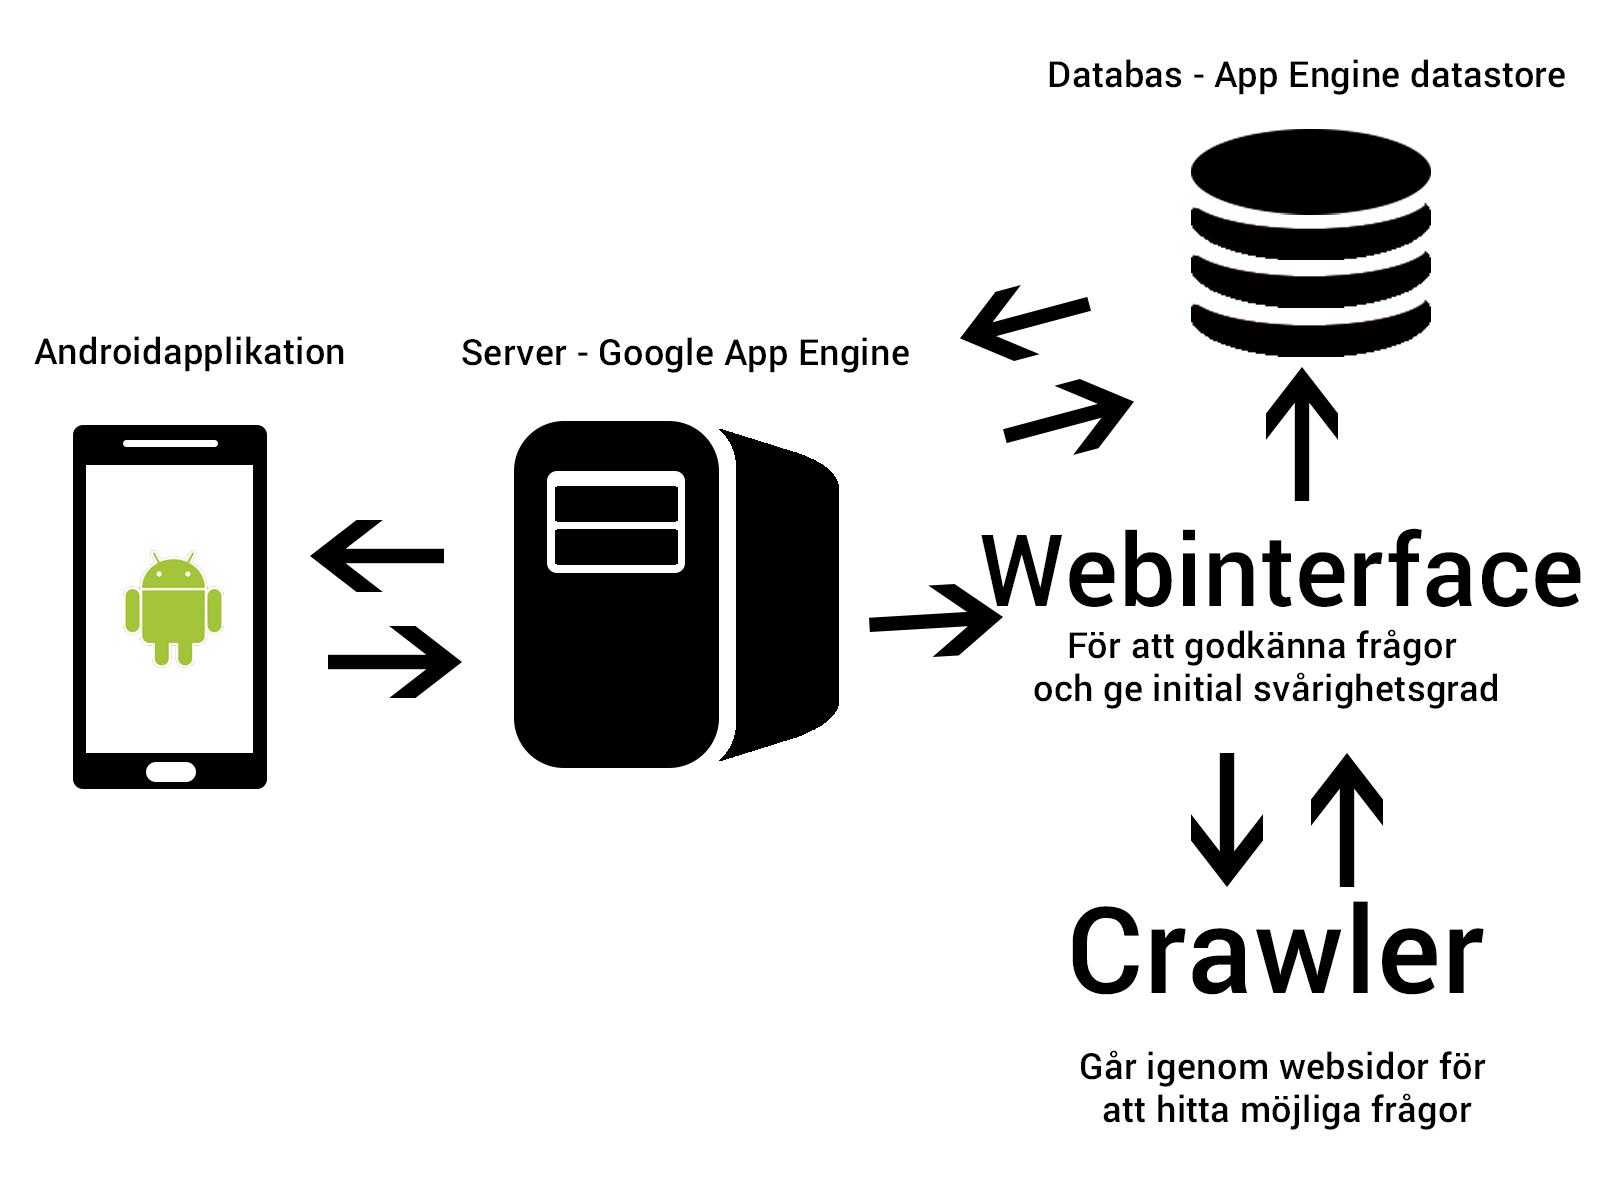
\includegraphics[width = \textwidth]{systemstruktur.jpg} 
	\end{centering}
	\caption{\textit{Illustration av systemstrukturen}}
\end{figure} 

\subsubsection{Androidapplikationen}
Androidapplikationen, vilket är klienten i systemet, är spelet som utvecklats. Det här är den del av systemet som användaren direkt ser och använder.

När det är den aktuella spelarens tur får denne en chunk med fem frågor och dess svar (årtal). Det är sedan klienten som rättar frågorna och därefter skickas svaren tillbaka till servern.
\subsubsection{Server}
Klienten kommunicerar med en server som körs i Google App Engine. Servern är utvecklad i programspråket Go (Golang) \cite{golang}. Servern agerar även som en brygga mellan klienten och den databas som används. När klienten kräver nya frågor till spelet kommunicerar servern med databasen som skickar frågorna till servern som i sin tur skickar vidare till klienten. Utöver kommunikation till klienten och databasen används även servern för att köra crawlern som är den automatiska informationshämtaren. Servern har också till uppgift att med jämna mellanrum köra fråge- och användarbalanseringssystemet som justerar svårighetsgraden på frågorna respektive spelarna i systemet. 
\subsubsection{Databas}
Databasen som servern kommunicerar med körs, likt servern, i App engine med biblioteket \textit{datastore}. Datastore är Google App Engines egna hantering av data, systemet hanterar datalagring med både SQL och noSQL.
\subsubsection{Crawler}
Inbyggt i servern finns en form av crawler som hanterar semi-automatisk informationshämtning av frågematerial. Hela systemet syftar till att via en given länk läsa igenom den länkade sidan och dess undersidor för att hitta information som passar som frågor för spelet. 

Sidor som har visat sig vara relativt enkla att läsa in är Wikipedias undersidor av typen listningssidor. Den här typen av sidor har en punktlista med årtal samt en beskrivande mening av det årtalet inom den kategori som Wikipediasidan handlar om. Ett exempel är sidan som listar datorspelsår: \url{http://sv.wikipedia.org/wiki/Lista_%C3%B6ver_datorspels%C3%A5r}. Vid inläsning av den här typen av sida separeras helt enkelt varje <li>-element där ett bindestreck eller kolon förekommer och därefter sparas varje kombination av årtal och händelse i ett temporärt cache.

När alla  händelser har lästs in i cachet presenteras de inlästa händelserna en i taget i ett webinterface. Webinterfacet visar ett årtal, en fråga samt fyra knappar. Knapparna anger svårighetsgrad lätt, medel eller svår samt ett alternativ för att ta bort den aktuella frågan helt.

\begin{figure}[H]
	\begin{centering}
	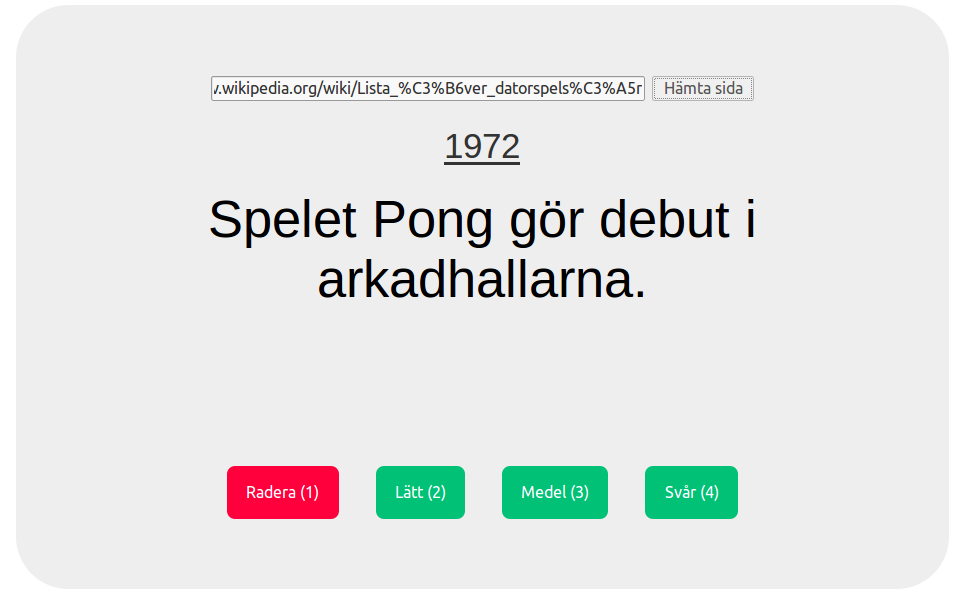
\includegraphics[width=\textwidth]{crawler} 
	\end{centering}
	\caption{\textit{Webinterface för crawlern}}
\end{figure}

De fyra knapparna är mappade till siffrorna 1-4 på tangentbordet för att det ska gå snabbt att klicka igenom frågorna. Texten är också redigerbar för att administratören snabbt ska kunna justera grammatiska fel.

\subsubsection{Balanseringssystemet}
Balanseringssystemet syftar till två saker, dels till att justera svårighetsgraden på frågorna som finns i databasen och dels till att justera spelarnas nivå. Efter varje avslutad match skickas alla frågor som var med i matchen samt båda spelarnas svar på respektive frågor. Utifrån detta justeras sedan nivåerna.

Om en spelare med låg nivå svarar rätt på en fråga så justeras frågans svårighetsgrad ner, ju högre nivå frågan har, desto större nedjustering sker. En spelare med hög nivå påverkar inte frågorna lika mycket som en spelare med låg nivå. Det här beror på att om en spelare med låg nivå svarar rätt på en svår fråga så är nivån på frågan förmodligen mycket mer felaktig än om en avancerad spelare svarat rätt på samma fråga. 

\begin{verbatim}
downDiff = int((1.0-(userRatio*questionRatio))*10.0)
\end{verbatim}

Kodsnutten ovan är ett exempel på en justering som sker om en spelare svarat rätt på den aktuella frågan. userRatio är ett värde mellan 0-1 på spelarens nivå (0 är nybörjare, 1 är avancerad). questionratio är ett värde mellan 0-1 på frågans nivå. downDiff är det värde som frågans nivå sänks med (mellan 0-10). 

\subsection{Avgränsningar}
En applikation för iOS prioriteras inte i första hand. Skulle det bli tid över och resten av systemet anses tillräckligt klart så kommer detta att utvecklas, men annars inte. Någon applikation för Windows finns inte heller med i planeringen. Spelet kommer troligtvis ha ett par kategorier som ska finnas med i spelet, men dessa är ännu inte valda. 

I applikationen finns det många funktioner som skulle vara roliga och användbara, men inför projektet hade vi några funktioner som ansågs vara viktiga att ha med. Den viktigaste funktionen är att kunna hitta och spela en match. En funktion för att hitta och hantera vänner man har i spelet och även kunna se statistik över matcherna man spelat mot en vän. Dessa funktioner behöver så klart även implementeras på server.

\subsection{Krav}
Systemet ska klara många spelare samtidigt, dock bara två per spel. Någon speciell siffra är inte bestämd ännu men med tanke på den otroligt bra grunden för skalbarhet som projektet står på kommer en siffra för antal spelare ganska snart kunna bestämmas. Eftersom App Engine används för servern så kommer det inte bli något problem med den enkla förklaringen att det är en tjänst som automatiskt skalar med hänsyn på belastning. \cite{appenginescalability}

Informationssökaren ska tillsammans med den administrativa kontrollen ge frågor som håller hög kvalitet. En hög kvalitet betyder frågor som är relevanta och som följer den strukturen vi har tänkt oss. Frågorna ska vara lätta att läsa och förstå och samtidigt befinna sig i det breda spektrumet av svårighetsgrader vi kommer ha i spelet. Sökaren för frågorna ska också vara så pass bra att den administrativa kontrollen går fort och att så lite som möjligt behöver korrigeras efter att frågorna har samlats. För att applikationen inte ska kännas allderless för repititiv ska det finnas många frågor och av varierande art, det ska minst finnas 1000 frågor.

Designen av applikationen är något som är viktigt för oss, kravet i början var att han en inuitiv, responsiv och snygg design. Eftersom applikationen gjordes för Android skulle den också följa dess designmönster Material Design \cite{MaterialDesign}.

\subsection{Utvärdering}
Planen är att en fungerande beta eller alfaversion av systemet ska färdigställas ett tag innan projektets slut. I den här versionen ska användare ha möjlighet att ge feedback och att testa applikationen. Så många fel som möjligt ska sedan justeras innan den skarpa versionen släpps.

Gränssnittet och användandet av applikationen kommer också att utvärderas med hjälp av think aloud\cite{thinkaloud} och en heuristic evaluering \cite{heruistic}.

\newpage
\printbibliography[title={Referenser}]
\end{document}